\documentclass[norsk,a4paper,12pt]{article} 
\usepackage[norsk]{babel} 
\usepackage[T1]{fontenc} %for å bruke æøå 
\usepackage[utf8x]{inputenc} 
\usepackage{graphicx} %for å inkludere grafikk 
\usepackage{verbatim} %for å inkludere filer med tegn LaTeX ikke liker 
\usepackage{amsfonts} 
\usepackage{amsmath} 
\usepackage{amssymb} 
\usepackage{savesym} 
\savesymbol{square} 
%\bibliographystyle{plain} 
\usepackage{float} 
\usepackage{SIunits} 
\usepackage{textcomp} 
\usepackage{parskip} 
\usepackage{array} 
%\usepackage[framed]{mcode} 
\usepackage[margin=2.3cm]{caption}
\usepackage{listings}



\begin{document}
\title{AST 3310: Prosjekt 1}
\author{Peder Forfang}
\maketitle


\section{Rapport}

\subsection{Innledning}

Prosjekt 1 går ut på å modellere den innerste delen av solen. I kjernen til enhver stjerne blir energi og varme 
produsert gjennom fusjon av atomkjerner. Hvor effektivt fusjonen skjer er avhengig av temperaturen og trykket i 
kjernen til stjernen. Den produserte energien blir transportert til overflaten av ved hjelp av elektromagnetisk
 stråling eller varm gass som forflytter seg. Dette kan modelleres ved å løse ligningene 
som beskriver den indre strukturen i sola: 

(1)
\begin{align*}
 \frac{\partial r}{\partial m} = \frac{1}{4\pi r^2\rho}
\end{align*}
(2) 
\begin{align*}
\frac{\partial P}{\partial m} = -\frac{Gm}{4\pi r^4}
\end{align*}
(3)
\begin{align*}
 \frac{\partial L}{\partial m} = \varepsilon
\end{align*}
(4)
\begin{align*}
 P = P_G + P_{rad}
\end{align*}
(5) 
\begin{align*}
\frac{\partial T}{\partial m} = -\frac{3\kappa L}{256\pi^2\sigma r^4T^3}
\end{align*}

der $\varepsilon $ er energien utløst fra fusjonen i kjernen, $\kappa $ er opasiteten
og resten av symbolene har sin standard beskrivelse. I 
beregningene antar vi en ideell tilstandsligning og at alle elementer er fullt ionisert. 
Ødeleggelses raten til elementene skal ikke overskride produksjons raten,
 men bortsett fra det unnlater vi hvordan elementene i kjernen utvikler seg utenom PPI og PPII reaksjonen.

\subsection{Framgangsmåte}

Under prosjektet har jeg støtt på svært mange numeriske problemer, og jeg må desverre meddele at jeg ikke klarte å løse 
dem alle. Mesteparten av tiden har av denne grunn gått med til feilsøking. Jeg vil påpeke at jeg er fullt klar over 
mine mangler på numerisk klokskap, og blir ikke overrasket hvis problemene jeg har støtt på har åpenbare løsninger.
Denne rapporten er derfor mer fokusert på min 
fremgangsmåte til prosjektet og forklaring av koden enn resultater og fysiske forklaringer. 

$\varepsilon $ hentet jeg fra energifunksjonen jeg lagde i Prosjekt 0, der målet var å regne ut 
energien til PPI og PPII reaksjonene. Denne bød på
litt problemer. Mens verdiene fra reaksjonsraten til PPI kjeden og første ledd i PPII kjeden 
passer bra med ``sanity testen'' er de to siste leddene i PPII, henholdsvis $r_{e7} $ og $r_{17} $, totalt vannvid. 
Mitt første steg i dette prosjektet ble derfor å nøste opp denne knuten, desverre uten hell.   

Et utdrag fra koden. Her regnes 7Be + e reaksjonen.
\begin{lstlisting}
r_7e = lam_e7*n_Be*n_e/ro 	# lam_e7 hentet fra tabell 3.1
Q7e = 0.05E6*1.602176565E-19 	# [Joule]
E7e = r_7e*Q7e*ro
\end{lstlisting}

Outputen fra funksjonen blir uansett mest påvirket av variablene $\rho $ og T så for å fullføre programmet tar jeg 
likevel i bruk verdiene jeg får fra energi funksjonen. Neste steg er å lage 
en funksjon som løser ligningene (1), (2), (3), (4) og (5). Fra ideell gasslov fant jeg $\rho $

(6)
\begin{align*}
\rho = \frac{P[i]\mu m_u}{k_bT[i]}
\end{align*}

Med dette resultatet og initialverdier hentet fra oppgaveteksten regner funksjonen så ut ligningene

\begin{lstlisting}
dr_dm = 1./(4*pi*r[i]**2*ro)
dP_dm = - G*M[i]/(4*pi*r[i]**4)
dL_dm = E
dT_dm = -3.*k_SI*L[i]/(256*pi**2*sb*r[i]**4*T[i]**3)

M[i+1] = M[i] + dm
r[i+1] = dr_dm*dm + r[i]
P[i+1] = dP_dm*dm + P_r + P[i]
L[i+1] = dL_dm*dm + L[i]
T[i+1] = dT_dm*dm + T[i]

\end{lstlisting}

Der steglengden $\partial m $ er regnet ut ved å følge oppskriften i variablesteplength.pdf.
Den oppdateres for hver gang i loopen på en slik måte at den ikke overskrider akseptable verdier.

\begin{lstlisting}
 #finding dm
f1 = 1./(4*pi*r[i]**2*ro)
dm1 = abs(r[i]*0.01/f1)
dm_list.append(dm1)
f2 = abs(- G*M[i]/(4*pi*r[i]**4))
dm2 = P[i]*0.01/f2
dm_list.append(dm2)
f3 = abs(E)
dm3 = L[i]*0.01/f3
dm_list.append(dm3)
f4 = abs(-3.*k_SI*L[i]/(256*pi**2*sb*r[i]**4*T[i]**3))
dm4 = T[i]*0.01/f4
dm_list.append(dm4)
dm = -min(dm_list)
dm_list2[i] = dm
\end{lstlisting}

f1, f2, f3 og f4 er hendholdsvis ligning (1), (2), (3) og (5). $\partial m $ kan da regnes ut fra ligning

\begin{align*}
\partial m  = \frac{X_i*p}{f_i}
\end{align*}

der $X_i$ er verdien av r, P, L eller T som regnes ut og p er en skaleringsparameter. Jeg setter verdiene dm1, dm2..osv 
inn i en liste, finner minste verdi av disse, gjør den negativ og definerer den som $\partial m $.
Absoluttverdi tegnet er til for at verdiene skal ha riktig 
fortegn når jeg finner den minste verdien. På en slik måte beveger jeg meg innover mot stjernens senter.

Jeg er overbevist om at steglengden er hovedårsaken til problemene jeg har hatt. Fra en verdi på rundt $-10^{11} $ raser 
den mot null, slik at massen M så og si forblir konstant. Jeg rikker meg altså ikke av flekken!

Ved denne fremgangsmåten og disse verdiene får jeg startverdiene

\begin{lstlisting}
ro = 1.526e-13
E = 1.475e-15
dm = -8.083e+11
r = 3e+08
P = 1e+12
L = 4e+26
T =1e+05
M = 1e+30

\end{lstlisting}

og etter 10000 steg ender jeg på disse verdiene

\begin{lstlisting}
ro = 6.535e+08
E = 6.557e+33
dm = -4.034e-34
r = 3e-14
P = 5e+41
L = 4e+26
T =1e+13
M = 1e+30
\end{lstlisting}

Det er åpenbart noe som ikke stemmer. Ifølge ligning (2) er

\begin{align*}
 dP \propto \frac{M}{r^4}
\end{align*}

og siden massen M forblir konstant mens r går mot null vil P fly mot astronomiske høyder.
Noenlunde fornuftige verdier for P ville være rundt $P = 10^{15} $. Siden 

\begin{align*}
 \rho \propto \frac{P}{T}
\end{align*}

fører dette til en kjedereaksjon; energi $\rightarrow $ L $\rightarrow $ T går alle til himmels.
$\partial m $ er et resultat av alle disse variablene. 

En nærmere titt på kjøringen viser at $\partial m $ beveger seg over -1 allerede etter 911 kjøringer i loopen. Resultatene 
er da svært nære sine startverdier.

\begin{lstlisting}
 ro = 1.526e-13
E = 1.475e-15
dm = -1.011
r = 4e+04
P = 1e+12
L = 4e+26
T =1e+05
M = 1e+30
\end{lstlisting}

Ved å eliminere parene f1 og dm1, f2 og dm2 ...osv etter tur viser det seg at det eneste som påvirker $\partial m $ 
er f1 og dm1. Når jeg eliminerer disse blir $\partial m $ enormt stor, og massen M blir 0 etter bare 2 runder i 
loopen. 
Jeg har gjort noen forsøk på å erstatte $\partial m $ med konstant verdi, linspace og diverse andre metoder uten å
lykkes. 
Radiusen er muligens kjernen i problemet. Men jeg har ikke evnet å løse mysteriet.

\subsection{Siste ord}

Dette prosjektet endte ikke kanon bra for min del. Uten å ha fått noe særlig resultater sitter jeg igjen med en 
følelse av udugelighet og forvirring.
 Likevel håper jeg at jeg har fått fram at innsatsen var der, og selv om jeg ikke kom helt i mål har erfaringen 
vært nyttig. Jeg legger ved koden som fil, og hvis det skulle skjære seg legger jeg den også ved som tekst til slutt
 i denne rapporten. 

\begin{figure}[H] 
\begin{center} 
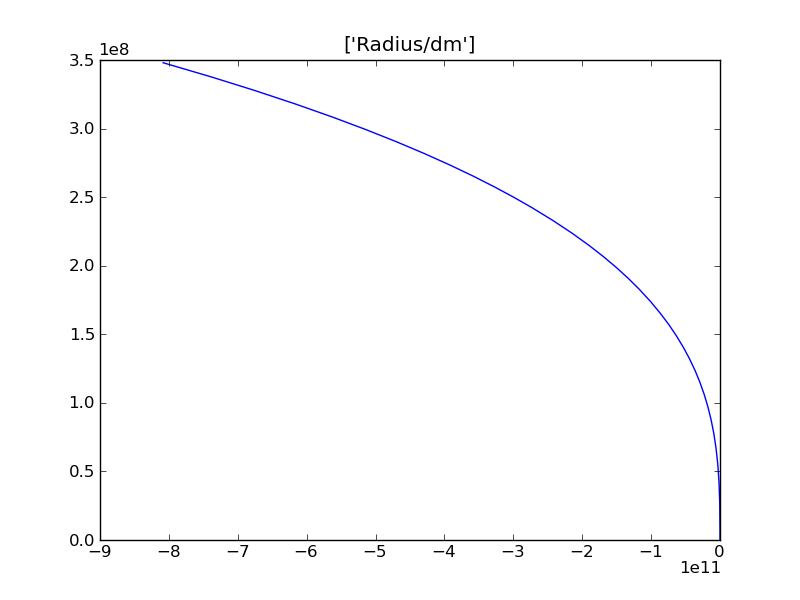
\includegraphics[scale=0.5]{r_dm.png} 
 

\caption{Ikke til å stole på.} 
\end{center} 
\end{figure}


\subsection{Kode}

\begin{lstlisting}
from numpy import *
import random

import pylab as plt
"""
Starting parameters
"""
L_0 = 3.846E26 # Luminosity [W]
R_0 = 0.5*6.96E8 # Radius [m]
M_0 = 0.7*1.989E30 # Mass [kg]
M_s = 1.989E30 # Mass sun [kg]
P_0 = 10E11 # Pressure [Pa]
ro_0 = 1E3 # Density [kg/m^3]
T_0 = 1E5 # Temperature [K]
T_c = 1.5E7*(M_0/M_s)**(1./3) #Core temperature [K]


X = 0.7 # Hydrogen
Y3 = 10**(-10) # Helium 3
Y = 0.29 # Helium 4
Z = 0.01 # Other metals
Z_Li = 10**(-13) # Lithium 7
Z_Be = 10**(-13) # Beryllium 7

m_u = 1.6605E-27 # Atomic mass unit [kg]

my = 1./(2*X +7*Y/4 +9*Z_Be/5 +9*Z/8)# average atomic weight
kb = 1.382E-23 # Boltzmans constant [m^2 kg/s^2 K]
c = 2.998E8 # Speed of light [m/s]
sb = 5.67E-8 # Stefan Boltzmann constant [W/m^2 K^4]
G = 6.672E-11 # Gravitaional constant [N m^2/kg^2]

Na = 6.02214129*10**23 # Avogadros konstant [1/mol]
V = 4/3*pi*R_0**3 # Volume
a = 4*sb/c

"""
#Reading the kappa values
"""

infile = open('opacity.txt', 'r')
lines = infile.readlines()
infile.close()

opacity = {}
first_line = lines[0]
logR = first_line.split()                               #the log(T) values
lgR = logR[1:]

R_list = []
for r in lgR:
	R = float(r)
        opacity[R] = {}
        R_list.append(R)


T_list = []
for line in lines[2:]:                                  
	words = line.split()
        logT =  (float(words[0]))                       
        T_list.append(logT)
        kappa = words[1:]

	for r, lgk in zip(lgR, kappa):
        	opacity[float(r)][logT] = float(lgk)    #




"""
 Energy function for PPI and PPII
"""
def supertrooper(ro, T, mu):
	# Densities of atomic species
	n_p = ro*X/(1*mu)
	n_He = ro*Y/(4*mu)
	n_e = (ro/2*mu)*(1 + X)
	n_d = ro*X/(2*mu)
	n_3He = ro*Y3/(3*mu)
	n_Li = ro*Z_Li/(7*mu)
	n_Be = ro*Z_Be/(7*mu)

	## Units of temperature
	T9 = T*1E9
	T_mongo = T9/(1+4.95*10**(-2)*T9)
	T_mongo2 = T9/(1+0.759*T9)

	## Reaction rates
	#2x H
	lam_pp = (4.01E-15*T9**(-2./3)*exp(-3.380/(T9**(1./3)))*(1 +
 0.123*T9**(1./3) + 1.09*T9**(2./3) + 0.938*T9))/Na*1E-6

	r_pp = lam_pp*n_p**2/ro
	Q1 = 0.15E6*1.602176565E-19 # Free energy [Joule]
	Q2 = 5.49E6*1.602176565E-19 # (From Deuterium reaction) 

	#2x 3He
	lam_33 = (6.04E10*T9**(-2./3)*exp(-12.276/(T9**(1./3)))*(1 +
 0.034*T9**(1./3) - 0.522*T9**(2./3) - 0.124*T9 + 0.353*T9**(4./3) +
 0.213*T9**(-5./3)))/Na*1E-6

	r_33 = lam_33*n_3He**2/ro
	Q3 = 12.86E6*1.602176565E-19 # Free energy [Joule]

	#3He 7Be
	lam_34 = (5.61E6*T_mongo**(5./6)*T9**(-3./2)*exp(-12.826*
T_mongo**(-1./3)))/Na*1E-6
	
	r_34 = lam_34*n_3He*n_He/ro
	Q4 = 1.59E6*1.602176565E-19 # Free energy [Joule]

	#7Be 7Li
	#lam_e7 = (1.34E-10*T9**(-1./2)*(1 - 0.537*T9**(1./3) + 
3.86*T9**(2./3) + 0.0027*T9**(-1.)*exp(2.515E-3*T9**(-1.))))/Na*1E-6
	lam_e7 = 1.34*10**(-10)*T9**(-0.5)*(1.0-0.537*T9**(1/3.)+
3.86*T9**(2/3.)+0.0027*T9**(-1.)*e**(2.515*10**(-3)*T9**(-1.)))/Na*1E-6
	r_7e = lam_e7*n_Be*n_e/ro
	Q7e = 0.05E6*1.602176565E-19 # Free energy [Joule]

	#7Li
	lamd_17 = (1.096E9*T9**(-2./3)*exp(-8.472*T9**(-1./3)) -
4.830E8*T_mongo2**(5./6)*T9**(-2./3)*exp(-8.472**T_mongo2**(-1./3)) + 
1.06E10*T9**(-2./3)*exp(-30.442*T9**(-1)))/Na*1E-6

	r_71 = lamd_17*n_Li*n_p/ro
	Q71 = 17.35E6*1.602176565E-19 # Free energy [Joule]	

	#7Be 8Be
	lam_17 = (3.11E5*T9**(-2./3)*exp(-10.262*T9**(-1./3)) + 
2.53E3*T9**(-3./2)*exp(-7.306*T9**(-1)))/Na*1E-6

	#14N 15O
	lam_p14 = (4.90E7*T9**(-2./3)*exp(-15.228*T9**(-1./3) - 
0.092*T9**2)*(1 + 0.027*T9**(1./3) - 0.778*T9**(2./3) - 0.149*T9 + 
0.261*T9**(4./3) + 0.127*T9**(5./3)) + 2.37E3*T9**(2./3)*exp(-
3.011*T9**(-1)) + 2.19E4*exp(-12.53*T9**(-1)))/Na*1E-6

	if r_7e > r_34:
		r_7e = r_34

	if r_71 > r_7e:
		r_17 = r_7e

	### Energy produced

	Epp = r_pp*(Q1 + Q2)*ro #PP
	E33 = r_33*Q3*ro #PPI
	E34 = r_34*Q4*ro	#PPII
	E7e = r_7e*Q7e*ro  #PPII
	E71 = r_71*Q71*ro  #PPII

	return Epp, E33, E34, E7e, E71



n = 10000

def evolution(r, ro, m, T, mu, dm):
	
	r = zeros(n)	
	r[0] = 0.5*6.96E8
	P = zeros(n)
	P[0] = P_0
	L = zeros(n)
	L[0] = 3.846E26
	T = zeros(n)
	T[0] = 1E5
	M = zeros(n)

	M[0] = M_0

	cnt = []
	ro_list = []
	ro_list.append(P_0*my*mu/(sb*T_0))
	dm_list2 = zeros(n)

	for i in range(n-1):
		counter = 1
		cnt.append(counter)
		
		ro = P[i]*my*mu/(sb*T[i])
		ro_list.append(ro)
	
		print 'ro = %.4g' % (ro)

		#Opacity
		logR = log10(ro*10**(-3)*10**6/T[i])
		logT = log10(T[i])
		LogR = min(R_list, key=lambda x:abs(x-logR))
		LogT = min(T_list, key=lambda x:abs(x-logT)) 

		lgk = float(opacity[LogR][LogT])                               
		k_SI = 10**(lgk-1)

		
		[Epp, E33, E34, E7e, E71] = supertrooper(ro, T[i], mu)
		E = Epp + E33 + E34 + E7e + E71
		print 'E = %.4g' % (E)

		dm_list = []

		#finding dm
		f1 = 1./(4*pi*r[i]**2*ro)
		dm1 = abs(r[i]*0.01/f1)
		dm_list.append(dm1)
		f2 = abs(- G*M[i]/(4*pi*r[i]**4))
		dm2 = P[i]*0.01/f2
		dm_list.append(dm2)
		f3 = abs(E)
		dm3 = L[i]*0.01/f3
		dm_list.append(dm3)
		f4 = abs(-3.*k_SI*L[i]/(256*pi**2*sb*r[i]**4*T[i]**3))
		dm4 = T[i]*0.01/f4
		dm_list.append(dm4)
		dm = -min(dm_list)
		dm_list2[i] = dm		

		#print 'dm = %.4g' % (dm)

		dr_dm = 1./(4*pi*r[i]**2*ro)
		#print 'r = %.g' % (r[i])

		dP_dm = - G*M[i]/(4*pi*r[i]**4)
		#print 'P = %.g' % (P[i])
		
		dL_dm = E
		#print 'dL_dm = %.g' % (dL_dm)	
		#print 'L = %.g' % (L[i])

		dT_dm = -3.*k_SI*L[i]/(256*pi**2*sb*r[i]**4*T[i]**3)
		#print 'dT_dm = %.g' % (dT_dm)
		#print 'T =%.g' % (T[i])
		
		P_r = (1./3)*a*T[i]**4 

		#print P_r
		
		M[i+1] = M[i] + dm
		#print 'M = %.g'% (M[i])
		if M[i+1] < 0:
			break


		r[i+1] = dr_dm*dm + r[i]

		P[i+1] = dP_dm*dm + P_r + P[i]
		
		L[i+1] = dL_dm*dm + L[i]

		T[i+1] = dT_dm*dm + T[i]
	print size(cnt)
	return r, P, L, T, M, dm_list2, ro_list

r, P, L, T, M, dm, ro = evolution(R_0, ro_0, m, T_0, m_u, dm)

plt.plot(dm,r)
plt.show()


\end{lstlisting}


\end{document}